
\project{Archimedes and $\pi$}

Let $A_n$ be the area of the regular $n$-gon inscribed in the unit
circle, and let $B_n$ be the area of the regular $n$-gon whose
inscribed circle has radius 1.  Figure~\ref{fig:03Archimedes} shows a
picture of $A_{n}$, $B_n$ (and $\pi$) for $n=4, 6, 12$.

\begin{figure}[b]
  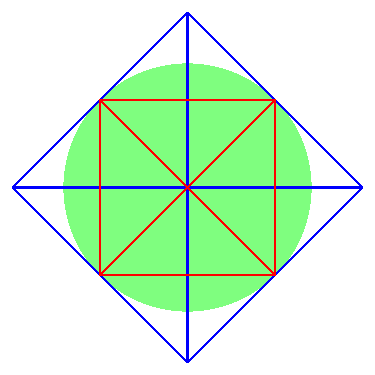
\includegraphics[width=0.3\textwidth]{03archimedes004.pdf}
  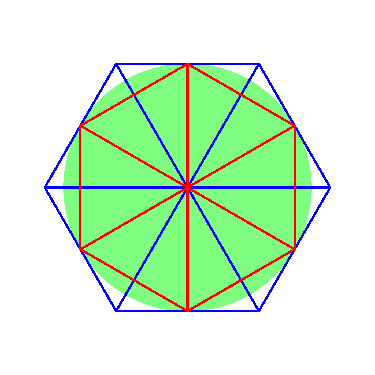
\includegraphics[width=0.3\textwidth]{03archimedes006.pdf}
  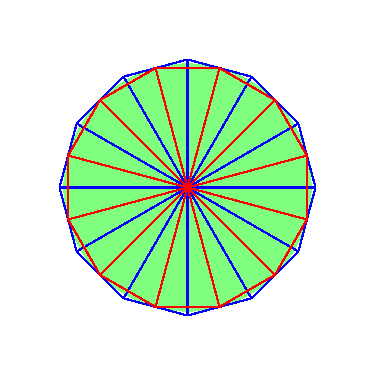
\includegraphics[width=0.3\textwidth]{03archimedes012.pdf}
  \caption{\textbf{Archimedes' approximations of $\pi$. } Archimedes
  approximated the area of a circle by calculating the areas of the
  inscribed (red) and circumscribed (blue) regular polygons with $n$ sides.  The
  larger $n$, the better the approximation.  Shown are the
  polygons for $n=4, 6$ and $12$.  Archimedes managed to compute
  $A_{96}$ and $B_{96}$ and by doing this got the most accurate
  approximation for $\pi$ that was known in his time.  See
  problem~\ref{ex:archimedes}.
  %See also:\\
  %{\small\url{http://www-history.mcs.st-andrews.ac.uk/HistTopics/Pi_through_the_ages.html}}
  }
  \label{fig:03Archimedes}
\end{figure}

\subprob Show that $A_n < \pi < B_n$.

\subprob Show that
\[
A_n = n \sin\frac{\pi}{n} \cos\frac{\pi}{n}
\]
and
\[
B_n = n \tan\frac\pi n.
\]

\subprob Compute $A_n$ and $B_n$ for $n=4$ and $6$ (exact answers,
without using a calculator).

\subprob Compute $\lim_{n\toi}A_n$ and $\lim_{n\toi}B_n$.
Note that there are (at least) two ways of getting an answer to this.
On one hand you can use the interpretion of $A_n$ and $B_n$ as areas
of polygons, and figure out what happens to those areas as
$n\to\infty$.  On the other hand, you could ignore the geometric
meaning of $A_n$ and $B_n$ and use \ref{eq:03trig-limit} with
$\theta = \pi/n$.

\subprob Archimedes computed both $A_{96}$ and $B_{96}$ and concluded
that $\pi$ must be somewhere between the values he found for $A_{96}$
and $B_{96}$.  To see how good Archimedes' approximation is, estimate
$A_{96}/B_{96}$.  You could use the formulas from part (b) to compute
$A_n/B_n= \cdots$ and then use
\eqref{eq:03sine-theta-is-roughly-theta} to approximate Sines and/or
Cosines that show up (use $\pi\approx 3$).
